	
	\subsection*{1.}
	
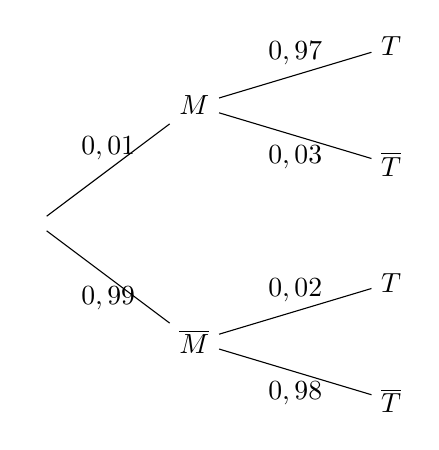
\begin{tikzpicture}
	[level 1/.style={level distance=2cm,
		sibling distance=3cm},
	level 2/.style={level distance=2.5cm,
		sibling distance=1.5cm}]
	\node {} [grow'=right]
	child {node {$M$}
		child {node {$T$}
			edge from parent node[above] {$0,97$}
		}
		child {node {$\overline T$}
			edge from parent node[below] {$0,03$}
		}
		edge from parent node[above] {$0,01$}
	}
	child {node {$\overline M$}
		child {node {$T$}
			edge from parent node[above] {$0,02$}
		}
		child {node {$\overline T$}
			edge from parent node[below] {$0,98$}
		}
		edge from parent node[below] {$0,99$}
	}
	;
\end{tikzpicture}
	
	\subsection*{2.}
	
	
	On a \(P(M \cap T) = P(M) \times P_M(T) = 0,01 \times 0,97 = 0,0097\).
	
	\subsection*{3.}
	
	D'après la loi des probabilités totales :
	
	\[ P(T) = P(M \cap T) + P(\bar{M} \cap T) \]
	
	Or,
	
	\[ P(\bar{M} \cap T) = P(\bar{M}) \times P_{\bar{M}}(T) = 0,99 \times 0,02 = 0,0198 \]
	
	Donc,
	
	\[ P(T) = 0,0097 + 0,0198 = 0,0295 \]
	
	\subsection*{4.}
		
	
	\[ P_T(M) = \dfrac{P(T \cap M)}{P(T)} = \dfrac{P(M \cap T)}{P(T)} = \dfrac{0,0097}{0,0295} \approx 0,32881 \]
	
	Donc,
	
	\[ P_T(M) \approx 0,3288 \text{ au dix-millième près.} \]
	
	\subsection*{5.}
	
		La réponse est non puisque 1 \% de la population est malade et que plus de 3 \% sont positives au test. De même, une personne malade peut être négative au test :
	
	\[ P(M \cap \bar{T}) = 0,01 \times 0,03 = 0,0003 \]
	
